%\documentclass[titlepage]{jsarticle}

%\usepackage[dvipdfmx]{graphicx}

%数式用パッケージ
%\usepackage{amsmath, amssymb}
%\usepackage{mathtools}
%\usepackage{cancel}
%\usepackage{cases}
%\usepackage{bm}
%\usepackage{array,booktabs}
%\usepackage{float}

%\usepackage{subcaption}

%ファインマングラフ用パッケージ
%\usepackage{feynmf}



%\graphicspath{{./figure/}}

%\begin{document}

 \subsubsection{プラスチックシンチレータのエネルギー較正}
 以下のようにして宇宙線を用いてエネルギー較正を行った.
 
 暗箱にプラスチックシンチレータを固定した状態で,本実験のときのe$^{+}$の入射面が上向きになるように床に置いて測定を行った.
 WFDのチャンネルトリガーを用いて全チャンネルのORでトリガーをとり,ゲートを208 ns にしてデータをとった.
 このときのトリガーのしきい値は全チャンネルで共通にしていて,電圧値は各チャンネルのレートが約3〜5 Hzになるように選んだ.
 各PMTにかけた電圧を表\ref{PS_PMT_HV}に示す.
 本実験においても表\ref{PS_PMT_HV}と同じ電圧値を用いて測定を行った.
 \begin{table}[H]
  \caption{プラスチックシンチレータ用のPMTのHV値}
  \label{PS_PMT_HV}
  \begin{center}
   \begin{tabular}{cc}\toprule
    PMT名&HV値 \\ \hline
    チャンネル0(あけみ)&-1600V \\
    チャンネル1(勝太郎)&-1418V \\
    チャンネル2(畑さん)&-1940V \\
    チャンネル3(紗智子)&-1762V \\
    チャンネル4(蘭)  &-1871V \\
    チャンネル5(矢部) &-1947V \\
    チャンネル6(政子) &-1980V \\
    チャンネル7(王)  &-1905V \\ \bottomrule
   \end{tabular} 
  \end{center}
 \end{table}%

 各チャンネル毎の電荷量のヒストグラムは図\ref{cosmicray}のようになった.
 ヒストグラム中の3つのピークの由来を左からそれぞれペデスタル,環境放射線,宇宙線と考えた.
 そのうち,宇宙線によるピークの部分をランダウ関数をガウシアンでたたみ込み積分した関数でフィッティングしてランダウ関数の最頻値を求めた.
 ガウシアンでたたみ込み積分をしたのは,プラスチックシンチレータとPMTで測定されるエネルギーには比較的大きいゆらぎがあるからである.
 得られた最頻値をエネルギー損失12 MeV に対応する電荷量とした.
 ただし,最頻値に対応するエネルギー損失の見積もりには次の2つの仮定を基にしている;
 \begin{itemize}
  \item プラスチックシンチレータに入射した宇宙線ミューオンのエネルギー損失は$dE/dx\sim 2 \mathrm{ MeV /cm}$である.
  \item 最頻値をとるのは宇宙線がシンチレータの底面に対して垂直に入射したとき,すなわち1層を通過するときの飛跡の長さが6 cmのときである.
 \end{itemize}
 この仮定から,1層でのエネルギー損失の最頻値は$2\mathrm{ MeV /cm}\times6\mathrm{ cm} = 12\mathrm{ MeV }$に対応すると判断した.
 さらにペデスタルをガウシアンでフィットしてエネルギーの0点に対応する電荷を求めた.
 図\ref{PS_calib}はこれら2点を用いて較正直線を求めた図である.
 \begin{figure}[H]
  \centering
  \includegraphics[height = 0.9\columnwidth , angle = -90]{figure/ikemitsu/cosmicray.pdf}
  \caption{宇宙線測定で得られたヒストグラム.横軸は電荷の積分値(pc)を表す.}
  \label{cosmicray}
 \end{figure}%
 \begin{figure}[H]
  \centering
  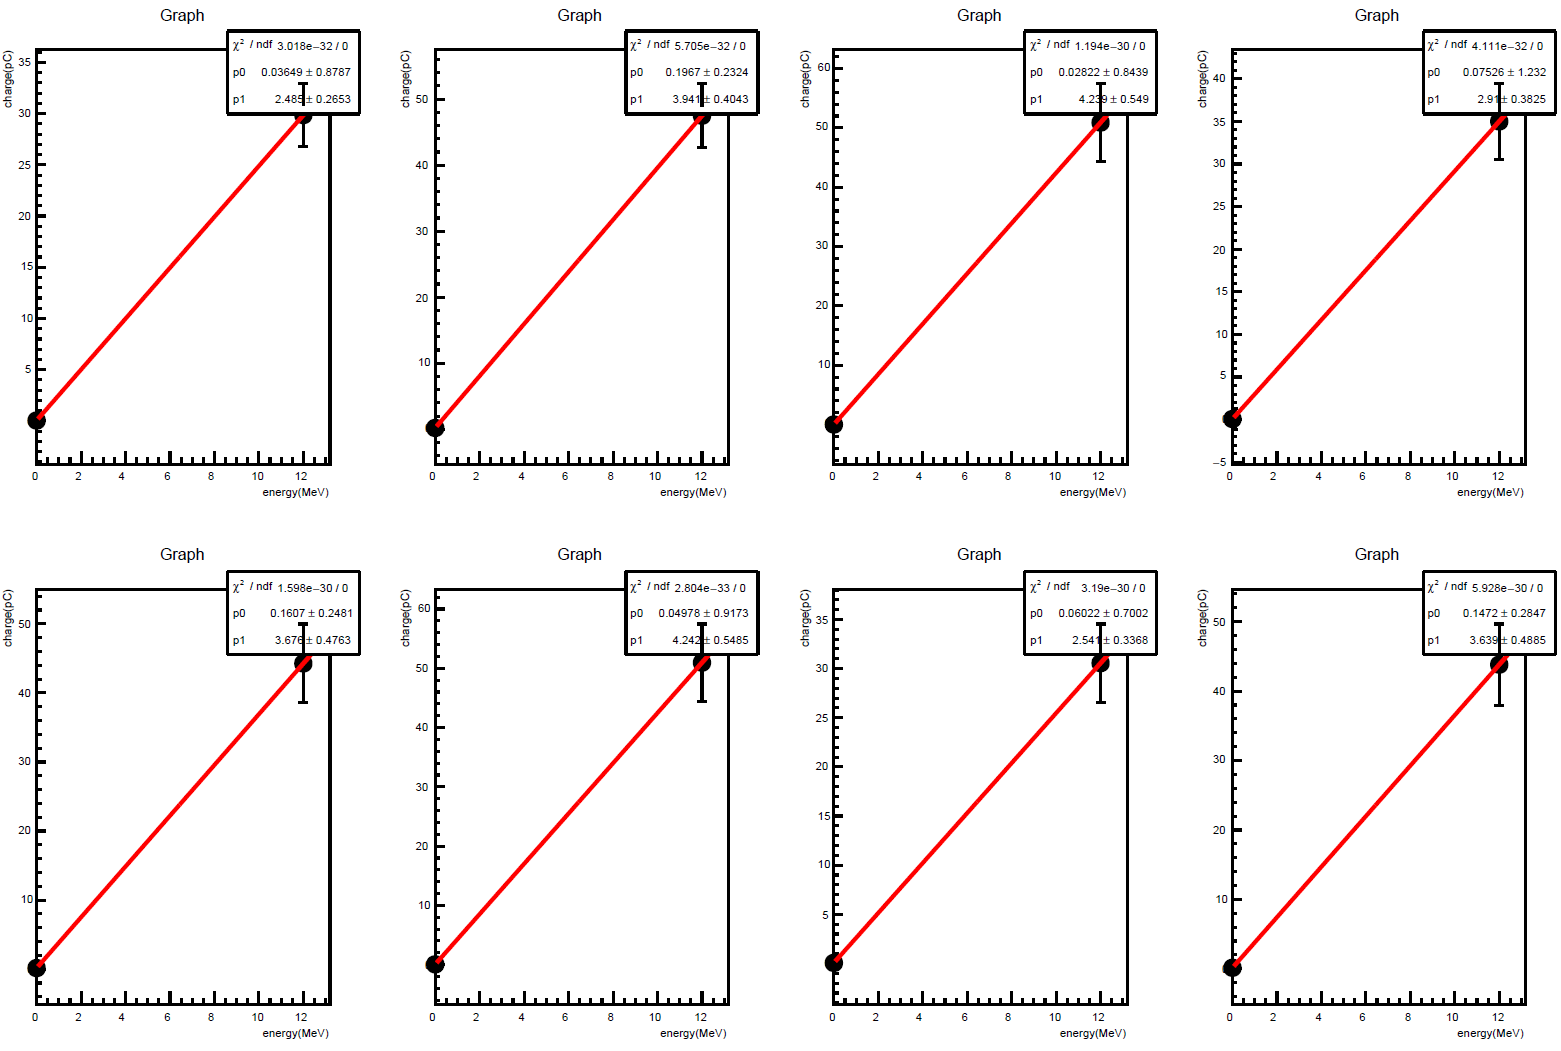
\includegraphics[height=0.9\columnwidth,angle=-90]{figure/ikemitsu/fit_calibline.pdf}
  \caption{較正直線のフィッテング}
  \label{PS_calib}
 \end{figure}%

 キャリブレーションの結果は表\ref{PS_calib_table}のようになった.
 表中のaとbは,エネルギー$E$と電荷$Q$の対応を$E = \mathrm{a}Q + \mathrm{b}$としたときの定数である.
 \begin{table}[h]
  \caption{キャリブレーションの結果}
  \label{PS_calib_table}
  \begin{center}
   \begin{tabular}{ccc}\toprule
    チャンネル番号&a &b \\ \hline
    0& 0.40$\pm$0.04 &0$\pm$0.3 \\
    1& 0.25$\pm$0.03 &0$\pm$0.06 \\
    2& 0.24$\pm$0.03 &0$\pm$0.2 \\
    3& 0.34$\pm$0.045 &0$\pm$0.4 \\
    4& 0.27$\pm$0.035 &0$\pm$0.07 \\
    5& 0.24$\pm$0.03 &0$\pm$0.21 \\
    6& 0.39$\pm$0.05 &0$\pm$0.3 \\
    7& 0.27$\pm$0.04 &0$\pm$0.08 \\ \bottomrule
   \end{tabular}
  \end{center}
 \end{table}%

 %%%%%%%%%%%%%%%%%%%池満パート開始%%%%%%%%%%%%%%%%%%%
 \section{プラスチックシンチレータで取得したデータの解析と考察}
 プラスチックシンチレータのデータの解析では波形解析やイベント選択の手法の異なる2つの解析手法を行った.それぞれで寿命と$g$因子の2つを求めた.
 以下ではそれぞれに解析手法Aと解析手法Bと名付けた.また,最後に両方の結果をまとめた.
 
  \subsection{解析手法A}
  プラスチックシンチレータ(以下,PS)検出器を用いて取得したデータを以下の方法で解析し,寿命,$g$因子,エネルギー分布を求めた.
  \begin{enumerate}
   \item イベントディスプレイから,初めの100 ns (50 Sample)の間は信号が来ていないことを確認し,0〜100 ns のデータの平均値をとってそれをbaselineとした.
   \item 信号のしきい値(threshold)の決定
	 \begin{itemize}
	  \item 宇宙線を用いた予備実験の結果から,12 MeV のエネルギーに対応する信号のピーク値を求めた.%宇宙線を用いた予備実験の説明は?? 12MeVがMIPがPSの厚さを通った時に落とすエネルギーである説明.
	  \item そのピーク値から,各チャンネルごとのthresholdを以下の値に決めた.
	  \item 寿命測定と$g$因子測定用には全層とも4 MeV 相当とした.threshold値の決め方についてはあとで述べる.
	  \item エネルギー測定用には,1層目にのみ4 MeV 相当のthresholdを設けた.2層目以降はthresholdを設けなかったのは,4 MeV 相当のthresholdを超えるエネルギーを持つイベントを全て取るためである.
	  %\item エネルギー測定用には,1層目:4 MeV 相当とし,2層目以降はthresholdを設けなかった.%なぜ?
	 \end{itemize}
   \item 各チャンネルごとで,thresholdを越えた時間を信号の時間(peaktime)とした.
   \item イベントディスプレイからおおよその信号の時間幅を決め,信号が検出されてから次の信号を検出するようになるまでのveto時間を40 ns にした.
   \item peaktimeから40 ns の間のデータを足すことで信号のchargeを求めた.
   \item 寿命と$g$因子について
	 \begin{itemize}
	  \item 各層の両側のチャンネルの信号のcoincidenceを取った.ただし,3層目は片側のみの信号である.
	  \item ここでcoincidenceの条件は,互いのpeaktimeが10 ns よりも近いものとした.
	  \item 寿命測定では,fingerを要求せずに層ごとのcoincidenceのみをとった.
	  \item $g$因子測定では,立体角を制限するために,層ごとだけでなくフィンガーカウンターとのcoincidenceを要求した.
	 \end{itemize}
   \item エネルギーについて
	 \begin{itemize}
	  \item 予備実験のデータから,各チャンネルごとにキャリブレーションをした.%上に同じ,実験説明が無い.
	  \item 各層のエネルギーとして,1,2,4層目では両側のチャンネルのエネルギーの平均を取り,3層目では片方のチャンネルのエネルギーを使用した.
	  \item fingerと1層目の両側のチャンネルの信号のcoincidenceをとり,そのときの全層のエネルギーの和を求めた.
		2層目以降のチャンネルで信号がない場合,そのチャンネルのエネルギーは0とした.
	  \item fingerとのcoincidenceを取ったのは,検出器の中心に入ったe$^{+}$の信号のみを選択するためである.
		電磁シャワーで生じたフォトンが検出器内で反応せずに外に漏れ出ると,検出されるエネルギーは実際のe$^{+}$のエネルギーよりも低い値になる.
		e$^{+}$が検出器の端の方に入射するときは検出器中央に入射するときより電磁シャワーによるフォトンが検出器の外に漏れやすいと考えた.
		以上のことから,fingerとのcoincidenceをとって検出器の中央に入射したイベントのみを解析に用いた.
	  %\item fingerとのcoincidenceを取ったのは,検出器の中心に入ったe$^{+}$の信号のみを選択し,エネルギー漏れを減らすためである.%エネルギー漏れとは?
	 \end{itemize}
  \end{enumerate}
  
  \subsubsection{信号検出のthreshold値について}
  信号検出時のthresholdの値の判断理由について触れておく.
  
  thresholdの値を1 MeV 相当から6 MeV 相当まで変化させて寿命を求めると,1 MeV 相当からthresholdが高くなるにつれて寿命は短くなり,4 MeV 相当以上のときに誤差の範囲で一定の値になった.
  このことから3 MeV 相当以下のthresholdでは低エネルギーのノイズを信号として処理していると考えた.
  よって,thresholdの値には4 MeV 相当の電圧値が妥当だと考えた.
  %1層目のthresholdを他層よりも高く設定しているのは,このようなバックグラウンドを除去するためである.%なぜ除去できる?
  %一方,寿命測定に関して,thresholdを上げてもfittingの結果は変わらず,統計誤差が大きくなるだけだった.%表現に違和感

  

  \subsubsection{得られた崩壊曲線とfittingの結果}
  図\ref{lt_layercoin}は,磁場なし標的を用いたときのミューオンの崩壊曲線である.
  それを次の$f_{\mathrm{life}}(t)$でfittingした結果が図\ref{lt_layercoin_fit}である.
  \begin{equation*}
   f_{\mathrm{life}}(t) = \exp[-(t+A)/\tau].
  \end{equation*}
  また,図\ref{g_layercoin}は磁場あり標的を用いたときのミューオンの崩壊曲線である.
  それを次の$f_{g}(t)$でfittingした結果が図\ref{g_layercoin_fit}である.
  \begin{equation*}
   f_{g}(t) = \exp[-(t+A)/\tau](1+B\cos(\omega t + \delta)).
  \end{equation*}
  
  fittingの範囲は1050 ns から7950 ns までとした. 
  今回使用したミューオンビームの分布はFWHM$\sim$100 ns ,すなわち$\sigma\sim$50 ns のガウス分布と考えることができる.
  図\ref{lt_layercoin}のヒストグラムがピーク値をとる約800 ns をガウシアンのピークだと考えて,その点から$5\sigma\sim 250$ns はfittingの対象外とした.
  また,ピークを検出してから40 ns のveto時間をとる解析方法から,8000 ns から後ろに40 ns 分は解析に用いることができない.
  以上のことからfitting範囲を決定した.
  
  fittingの結果は表\ref{fit_lt},\ref{fit_g}のようになった.表中の誤差はfittingに由来する統計誤差である.
  
  \begin{table}[H]
   \caption{寿命$\tau$のfitting結果}
   \label{fit_lt}
   \begin{center}
    \begin{tabular}{cc}\toprule
     coincidenceを取った層& $\tau$ (ns) \\ \midrule
     1 		        & 2223.7 $\pm$ 7.7 \\
     1+2 		& 2224 $\pm$ 10 \\
     1+2+3 		& 2217 $\pm$ 15 \\
     1+2+3+4 		& 2148 $\pm$ 35\\ \bottomrule
    \end{tabular}
   \end{center}
  \end{table}%
  
  \begin{table}[H]
   \caption{$g$因子のfitting結果}
   \label{fit_g}
   \begin{center}
    \begin{tabular}{cccc}\toprule
     coincidenceを取った層&$\tau$ (ns)& $\omega$ ($\times 10^{-3}$/ns) & $g$ \\ \midrule
     finger+1             &2170.4 $\pm$ 9.1 & $( 4.621 \pm 0.012 ) $ & 2.0091 $\pm$ 0.0054 \\
     finger+1+2 	  &2199 $\pm$ 13    & $( 4.614 \pm 0.011 ) $ & 2.0063 $\pm$ 0.0050 \\
     finger+1+2+3 	  &2205 $\pm$ 18    & $( 4.594 \pm 0.013 ) $ & 1.9973 $\pm$ 0.0055\\
     finger+1+2+3+4 	  &2142 $\pm$ 45    & $( 4.649 \pm 0.024 ) $ & 2.021 $\pm$ 0.011 \\ \bottomrule
    \end{tabular}
   \end{center}
  \end{table}%


  \begin{figure}[H]
   \centering
   \begin{subfigure}{\columnwidth}
    \centering
    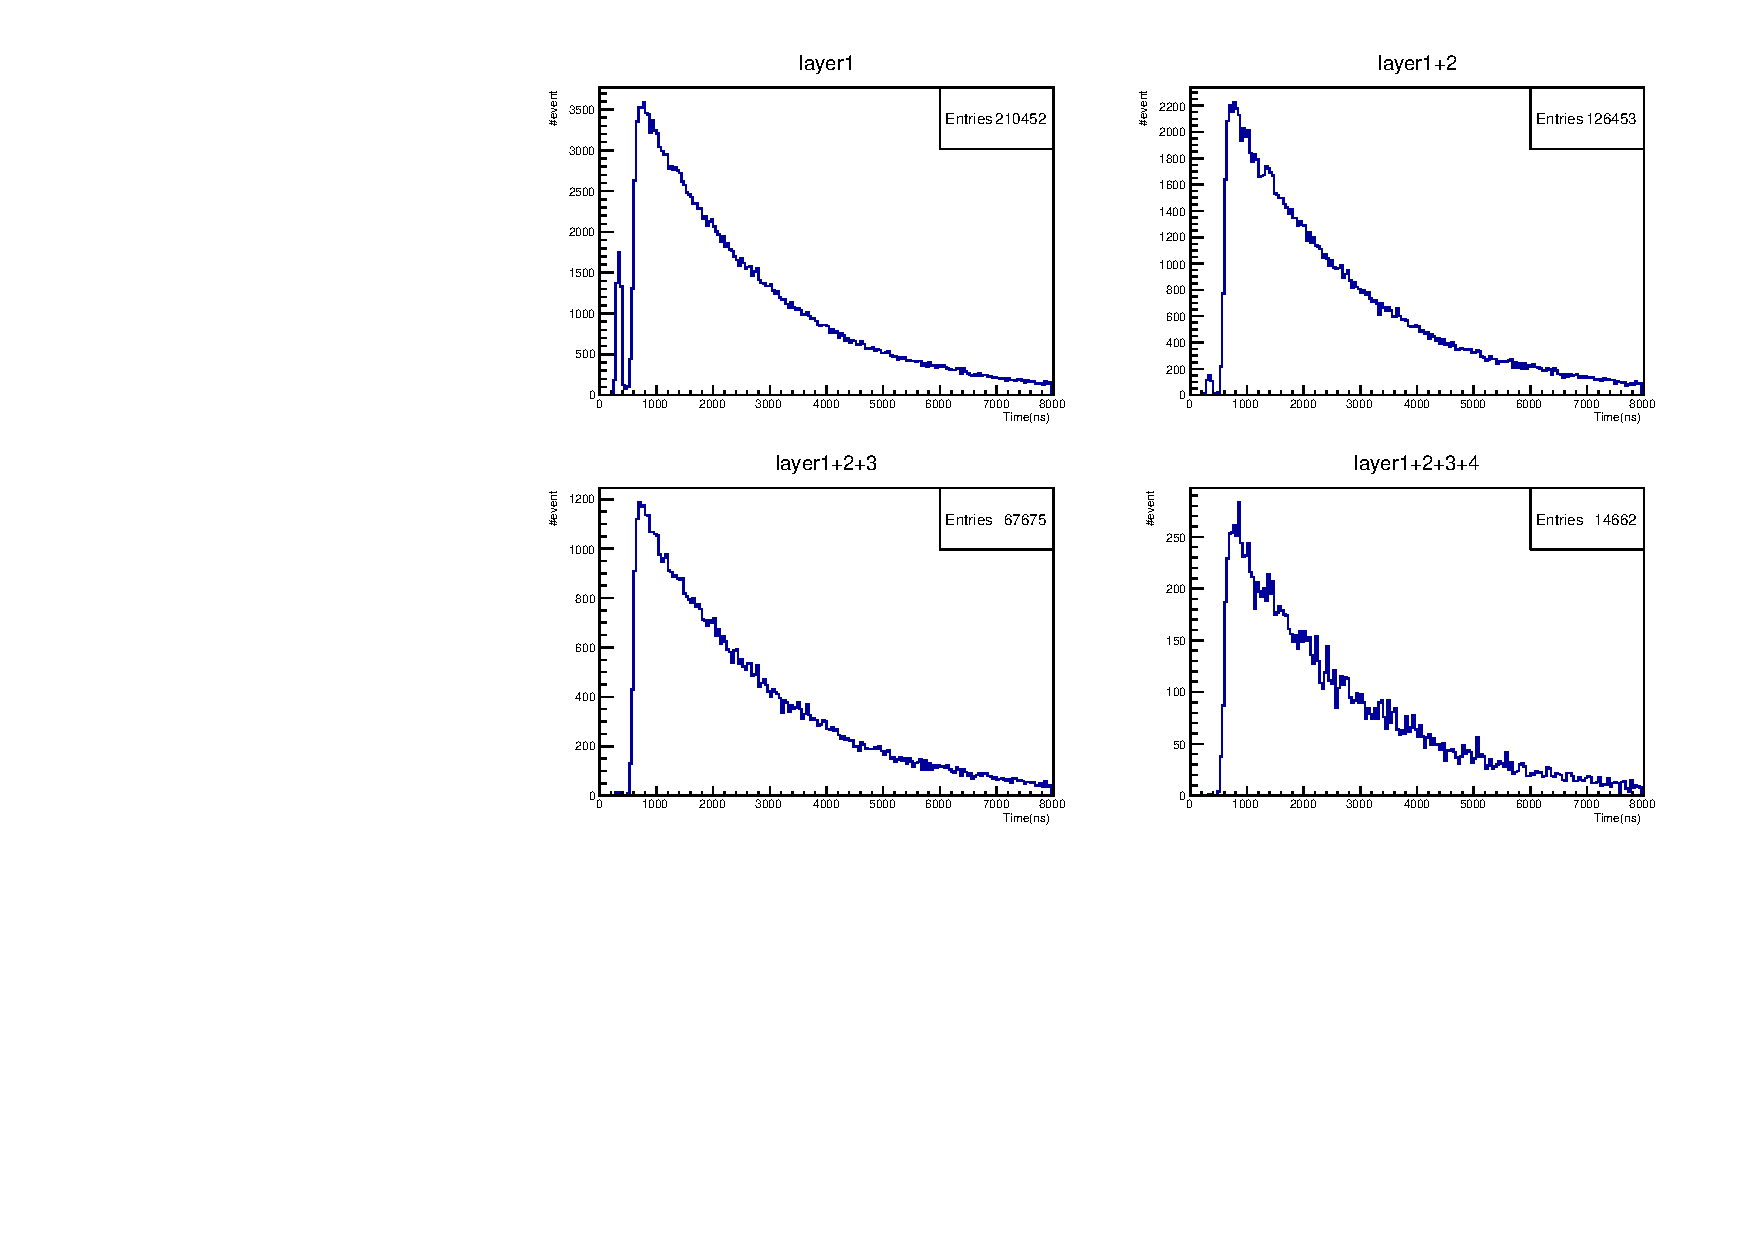
\includegraphics[height = 0.9\columnwidth , angle = -90]{figure/ikemitsu/lt_layercoin.pdf}
    \caption{層でcoincidenceを取って得られたヒストグラム(磁場なし標的)}
    \label{lt_layercoin}
   \end{subfigure}
   \begin{subfigure}{\columnwidth}
    \centering
    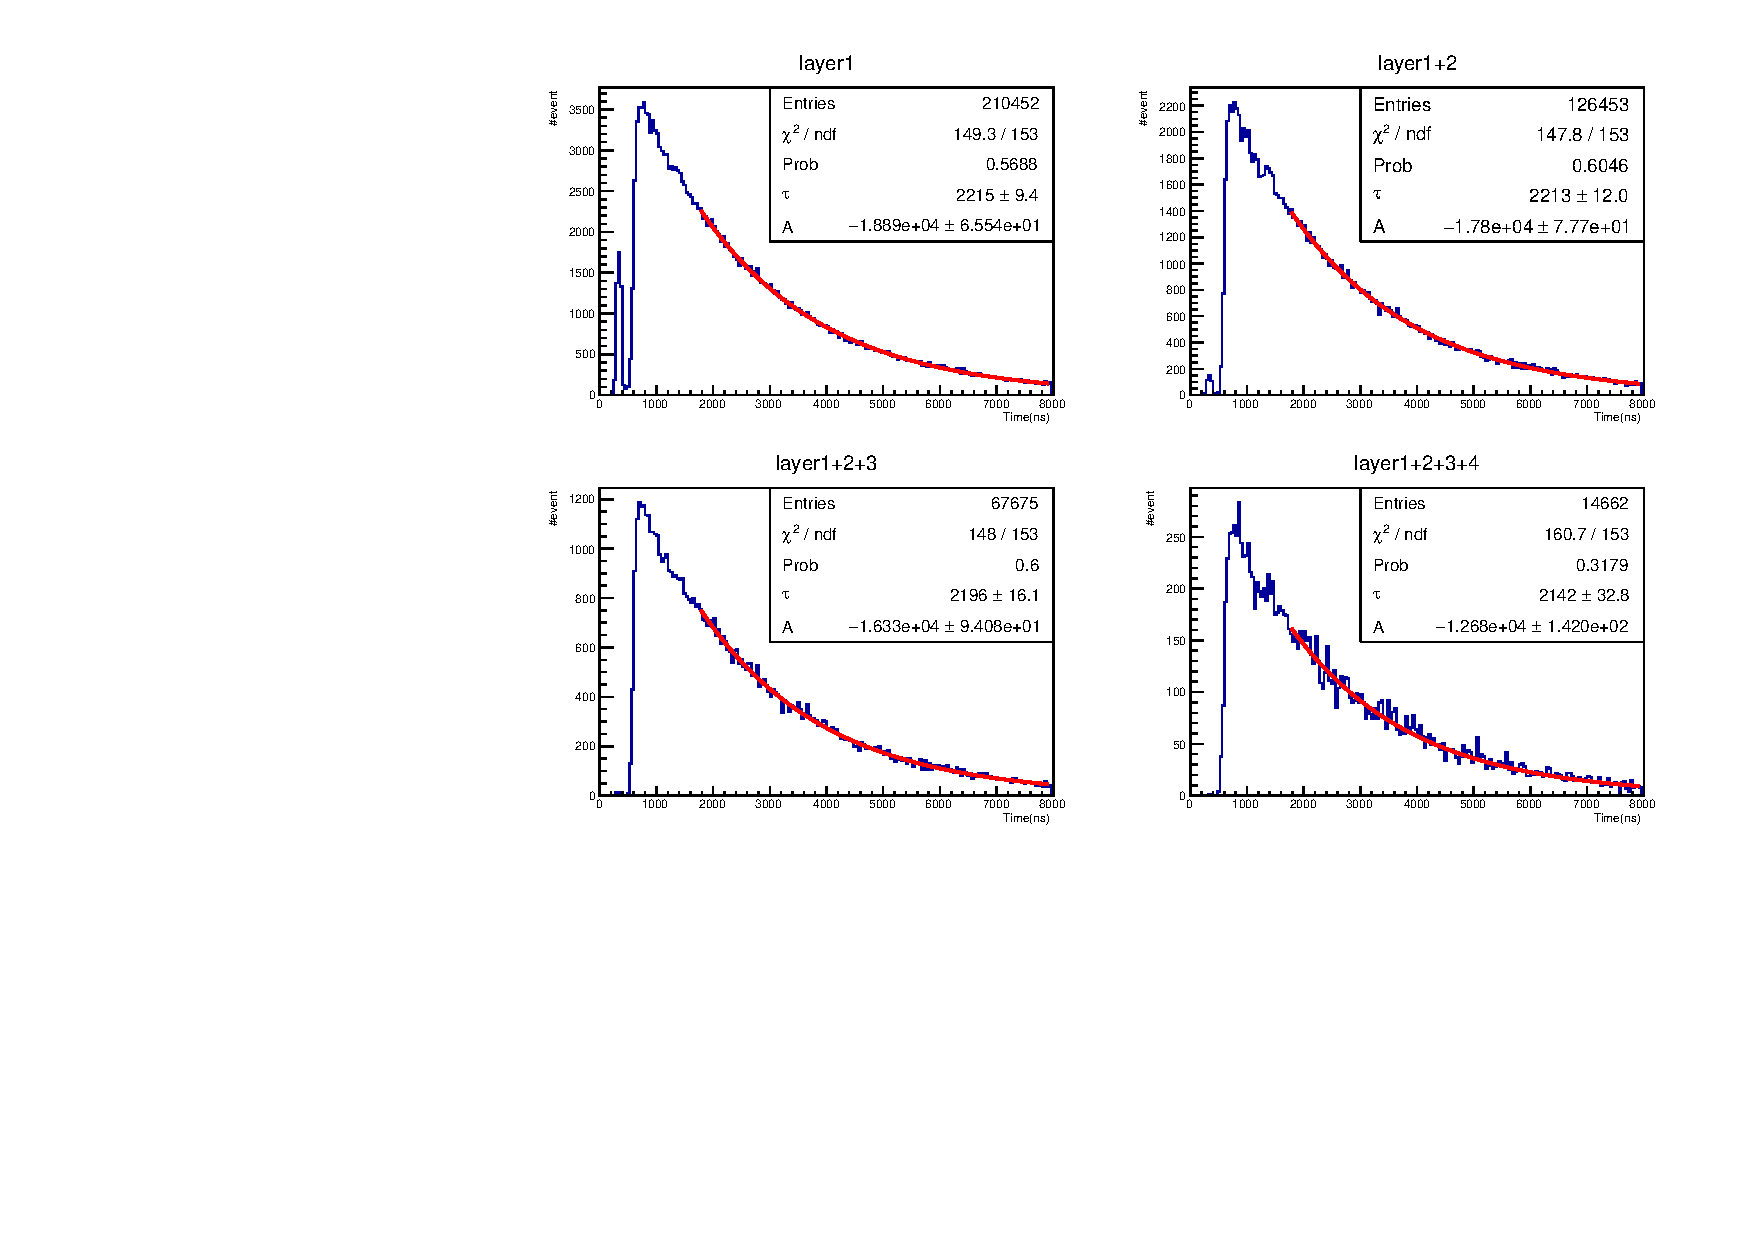
\includegraphics[height = 0.9\columnwidth , angle = -90]{figure/ikemitsu/lt_layercoin_fit.pdf}
    \caption{$f_{\mathrm{life}}(t)$でfittingをした図}
    \label{lt_layercoin_fit}
   \end{subfigure}
   \caption{fittingした図}
   \label{lt_layercoin_all}
  \end{figure}
  
  \begin{figure}[H]
   \centering
   \begin{subfigure}{\columnwidth}
    \centering
    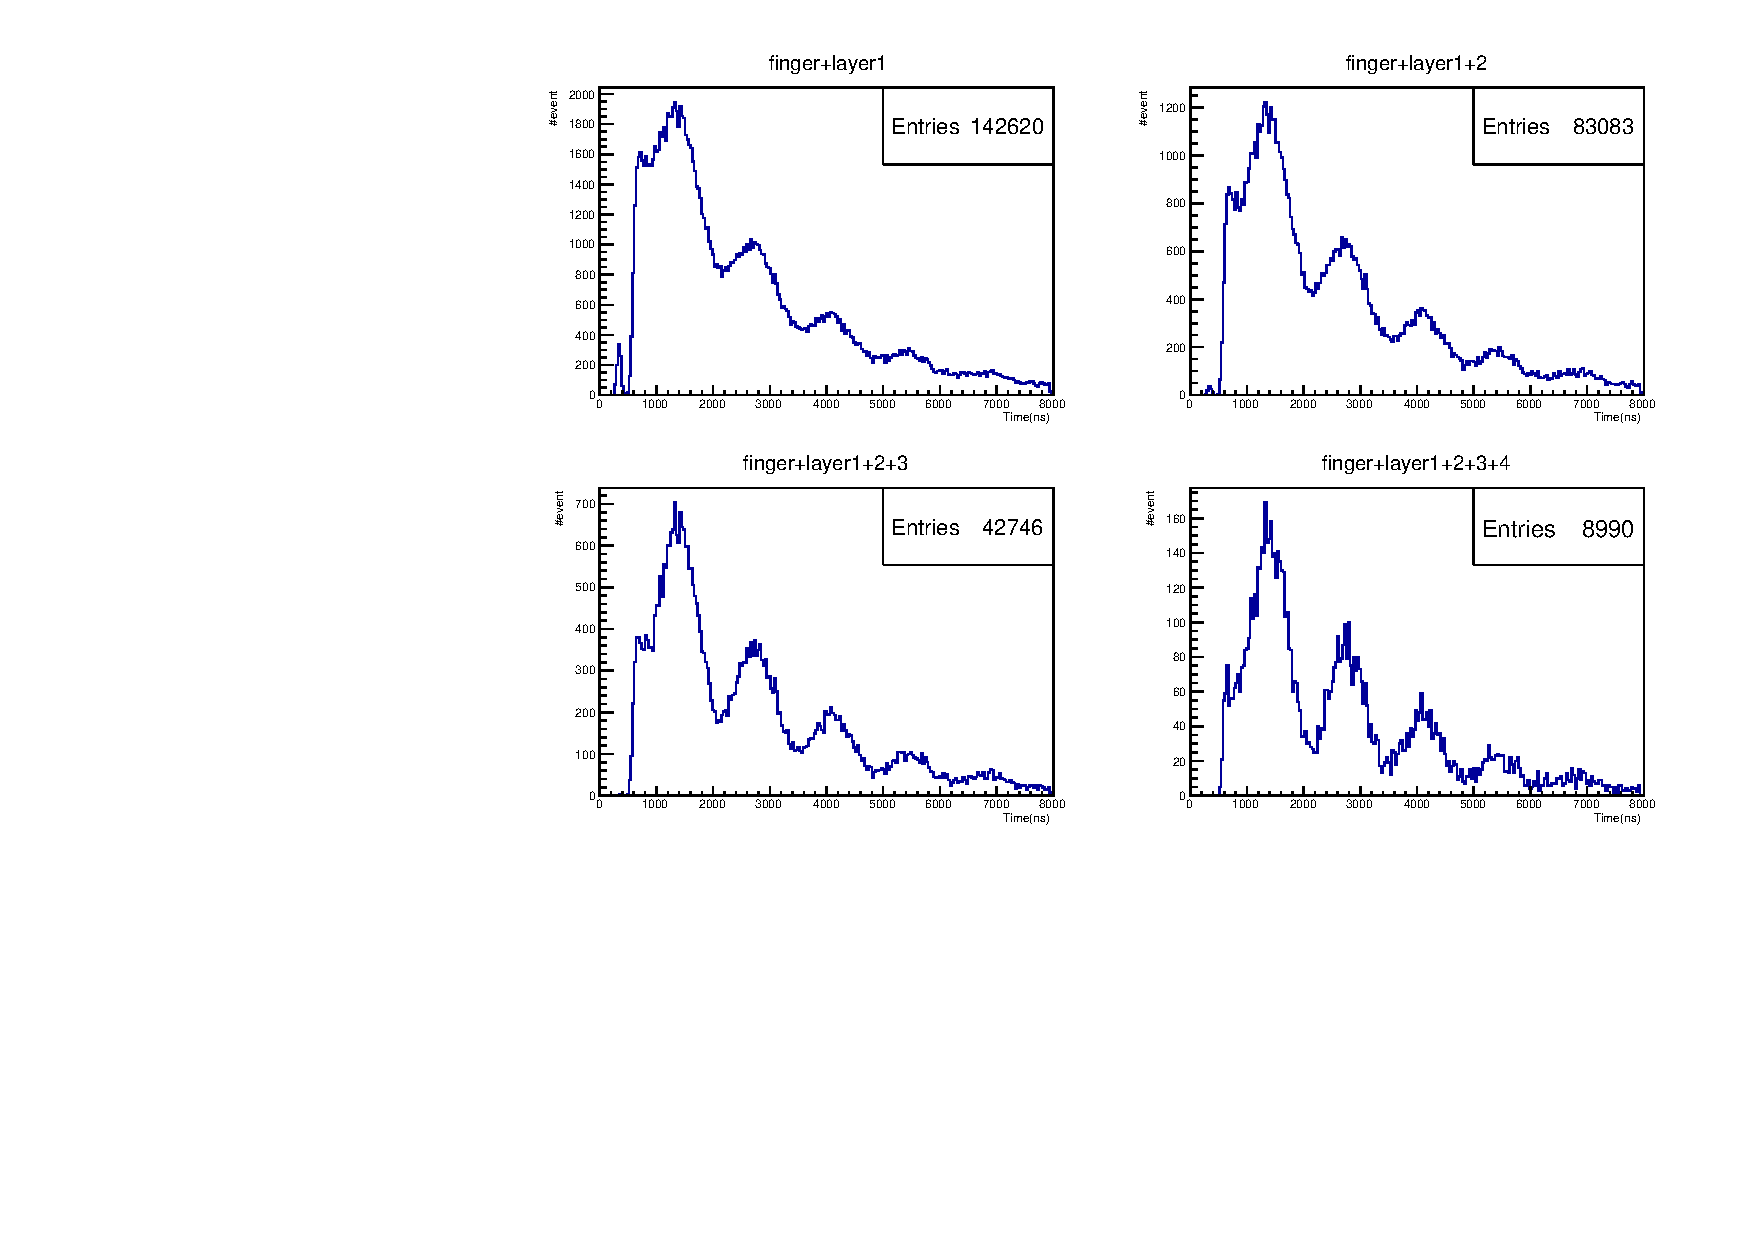
\includegraphics[height = 0.9\columnwidth , angle = -90]{figure/ikemitsu/g_layer_f_coin.pdf}
    \caption{層でcoincidenceを取って得られたヒストグラム(磁場あり標的)}
    \label{g_layercoin}
   \end{subfigure}
   \begin{subfigure}{\columnwidth}
    \centering
    \includegraphics[height = 0.9\columnwidth , angle = -90]{figure/ikemitsu/g_layer_f_coin_fit.pdf}
    \caption{$f_{g}(t)$でfittingをした図}
    \label{g_layercoin_fit}
   \end{subfigure}
   \caption{fittingした図}
   \label{g_layercoin_all}
  \end{figure}

  
    \subsubsection{fitting範囲の妥当性について}
  %よって,図\ref{lt_layercoin}のヒストグラムのピーク点は750 ns であるが,その点から1000 ns はfittingの対象外とし,%なぜ1000ns?
  %図\ref{lt_layercoin_fit}と図\ref{g_layercoin_fit}ではfittingの範囲を1750 ns から7950 ns までとした.
  上で述べたようにfittingの範囲は1050 ns から7950 ns としたが,この範囲の前側と後側で範囲を分けてfittingをすると,$\tau$と$g$の値は表\ref{fitrange1}〜\ref{fitrange4}のようになった.
  \begin{table}[H]
   \centering
   \begin{minipage}{0.4\columnwidth}
   \caption{寿命$\tau$;fitting範囲1050 ns 〜4550 ns }
   \label{fitrange1}
   \begin{center}
    \begin{tabular}{cc}\toprule
     coincidenceを取った層 & $\tau$ (ns) \\ \midrule
     1 			   & 2233 $\pm$ 14 \\
     1+2 		   & 2234 $\pm$ 19 \\
     1+2+3 		   & 2249 $\pm$ 27 \\
     1+2+3+4 	           & 2127 $\pm$ 63 \\ \bottomrule
    \end{tabular}
   \end{center}
   \end{minipage}
   \hspace*{5mm}
   \begin{minipage}{0.4\columnwidth}
    \caption{寿命$\tau$;fitting範囲4450 ns 〜7950 ns }
    \label{fitrange2}
    \begin{center}
     \begin{tabular}{cc}\toprule
      coincidenceを取った層 & $\tau$ (ns) \\ \midrule
      1 			   & 2250 $\pm$ 32 \\
      1+2 		   & 2238 $\pm$ 42 \\
      1+2+3 		   & 2257 $\pm$ 61 \\
      1+2+3+4 		   & 2013 $\pm$ 121 \\ \bottomrule
     \end{tabular}
    \end{center}   
   \end{minipage}
  \end{table}%

  \begin{table}[H]
    \caption{$g$因子;fitting範囲1050 ns 〜4550 ns }
    \label{fitrange3}
    \begin{center}
     \begin{tabular}{cccc}\toprule
      coincidenceを取った層&$\tau$ (ns)& $\omega$ ($\times 10^{-3}$/ns) & $g$ \\ \midrule
      finger+1             &2134 $\pm$ 15 & $( 4.638 \pm 0.020 ) $ & 2.0165 $\pm$ 0.0088 \\
      finger+1+2 	  &2185 $\pm$ 21 & $( 4.612 \pm 0.020 ) $ & 2.0054 $\pm$ 0.0085 \\
      finger+1+2+3 	  &2221 $\pm$ 32 & $( 4.615 \pm 0.021 ) $ & 2.0068 $\pm$ 0.0093\\
      finger+1+2+3+4 	  &2271 $\pm$ 87 & $( 4.663 \pm 0.040 ) $ & 2.028 $\pm$ 0.018 \\ \bottomrule
     \end{tabular}
    \end{center}    
  \end{table}%

  \begin{table}[H]
   \caption{$g$因子;fitting範囲4450 ns 〜7950 ns }
   \label{fitrange4}
   \begin{center}
    \begin{tabular}{cccc}\toprule
     coincidenceを取った層&$\tau$ (ns)& $\omega$ ($\times 10^{-3}$/ns) & $g$ \\ \midrule
     finger+1             &2254 $\pm$ 42 & $( 4.569 \pm 0.059 ) $ & 1.986 $\pm$ 0.026 \\
     finger+1+2 	  &2267 $\pm$ 58 & $( 4.618 \pm 0.053 ) $ & 2.008 $\pm$ 0.023 \\
     finger+1+2+3 	  &2245 $\pm$ 86 & $( 4.571 \pm 0.056 ) $ & 1.987 $\pm$ 0.024\\
     finger+1+2+3+4 	  &1975 $\pm$ 186& $( 4.64 \pm 0.11 ) $ & 2.016 $\pm$ 0.046 \\ \bottomrule
    \end{tabular}
   \end{center}
  \end{table}%

  表\ref{fitrange1}・表\ref{fitrange2}を表\ref{fit_lt}と比較し,
  表\ref{fitrange3}・表\ref{fitrange4}を表\ref{fit_g}と比較すると,fittingの範囲を変えても得られた$\tau$と$g$の値は各層ごとで誤差の範囲内で一致していると言える.
  このことから,fittingの範囲として1050 ns から7950 ns までは適切だと考えられる.
  %寿命に関して全層のcoincidenceがfittingの範囲が前半の時と後半の時とではコンシステントではない.系統誤差となるのでは?

  寿命に関して,全層でcoincidenceをとったときに3層目までよりも寿命が短くなっている.

  
  \subsubsection{エネルギー分布}
  磁場なし標的を用いたときのデータから求めたエネルギーのヒストグラムは図\ref{michel_PS}のようになった.
  ミューオンが散乱されて直接検出器に入射してくるイベントを除去するために,解析にはpeaktimeが1050 ns 以降のイベントのみを使用した.
  ガウシアンで入射してくるミューオンビームのピークと考えられる時間(800 ns 付近)から約$5\sigma$の間隔を開けることでビーム由来のミューオンはほぼ無視できると考えた.
  
  \ref{michel_PS}において横軸と縦軸の誤差としてそれぞれキャリブレーション由来のエネルギー分解能と統計誤差をつけたグラフが図\ref{michel_PS_gosa}である.
  %磁場なし標的を用いたときのデータから求めたエネルギー分布は図\ref{michel_PS}のようになった.
  %さらに,\ref{michel_PS}の各点において,キャリブレーションに由来するエネルギー分解能と統計誤差をそれぞれ横軸と縦軸の誤差として付けたのが図\ref{michel_PS_gosa}である.%図の縦軸の説明 2つの図で全然スケールが違うのはなぜ?
  \begin{figure}[H]
   \centering
   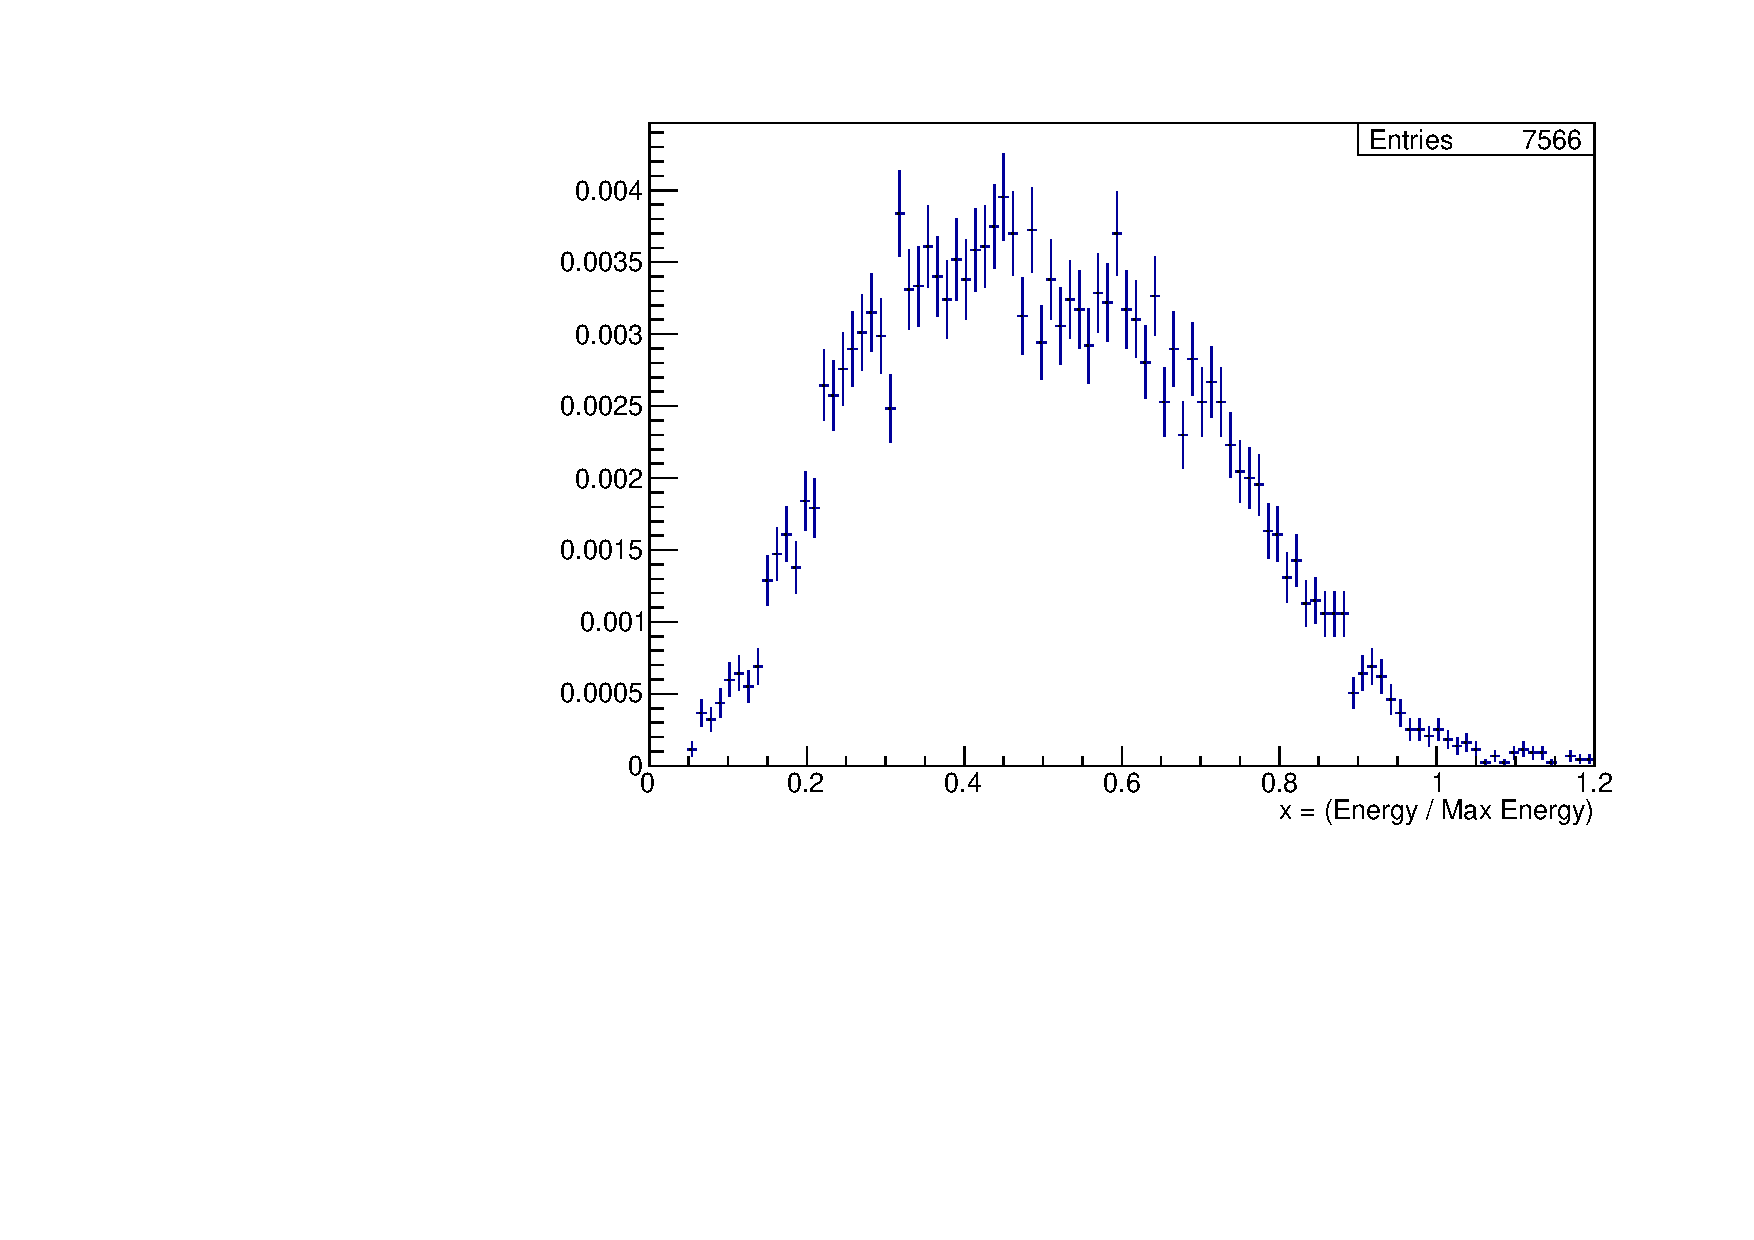
\includegraphics[height = 0.7\columnwidth , angle = -90]{figure/ikemitsu/michel_PS.pdf}
   \caption{PSで得られたエネルギー分布図;磁場なし標的}
   \label{michel_PS}
  \end{figure}
  
  \begin{figure}[H]
   \centering
   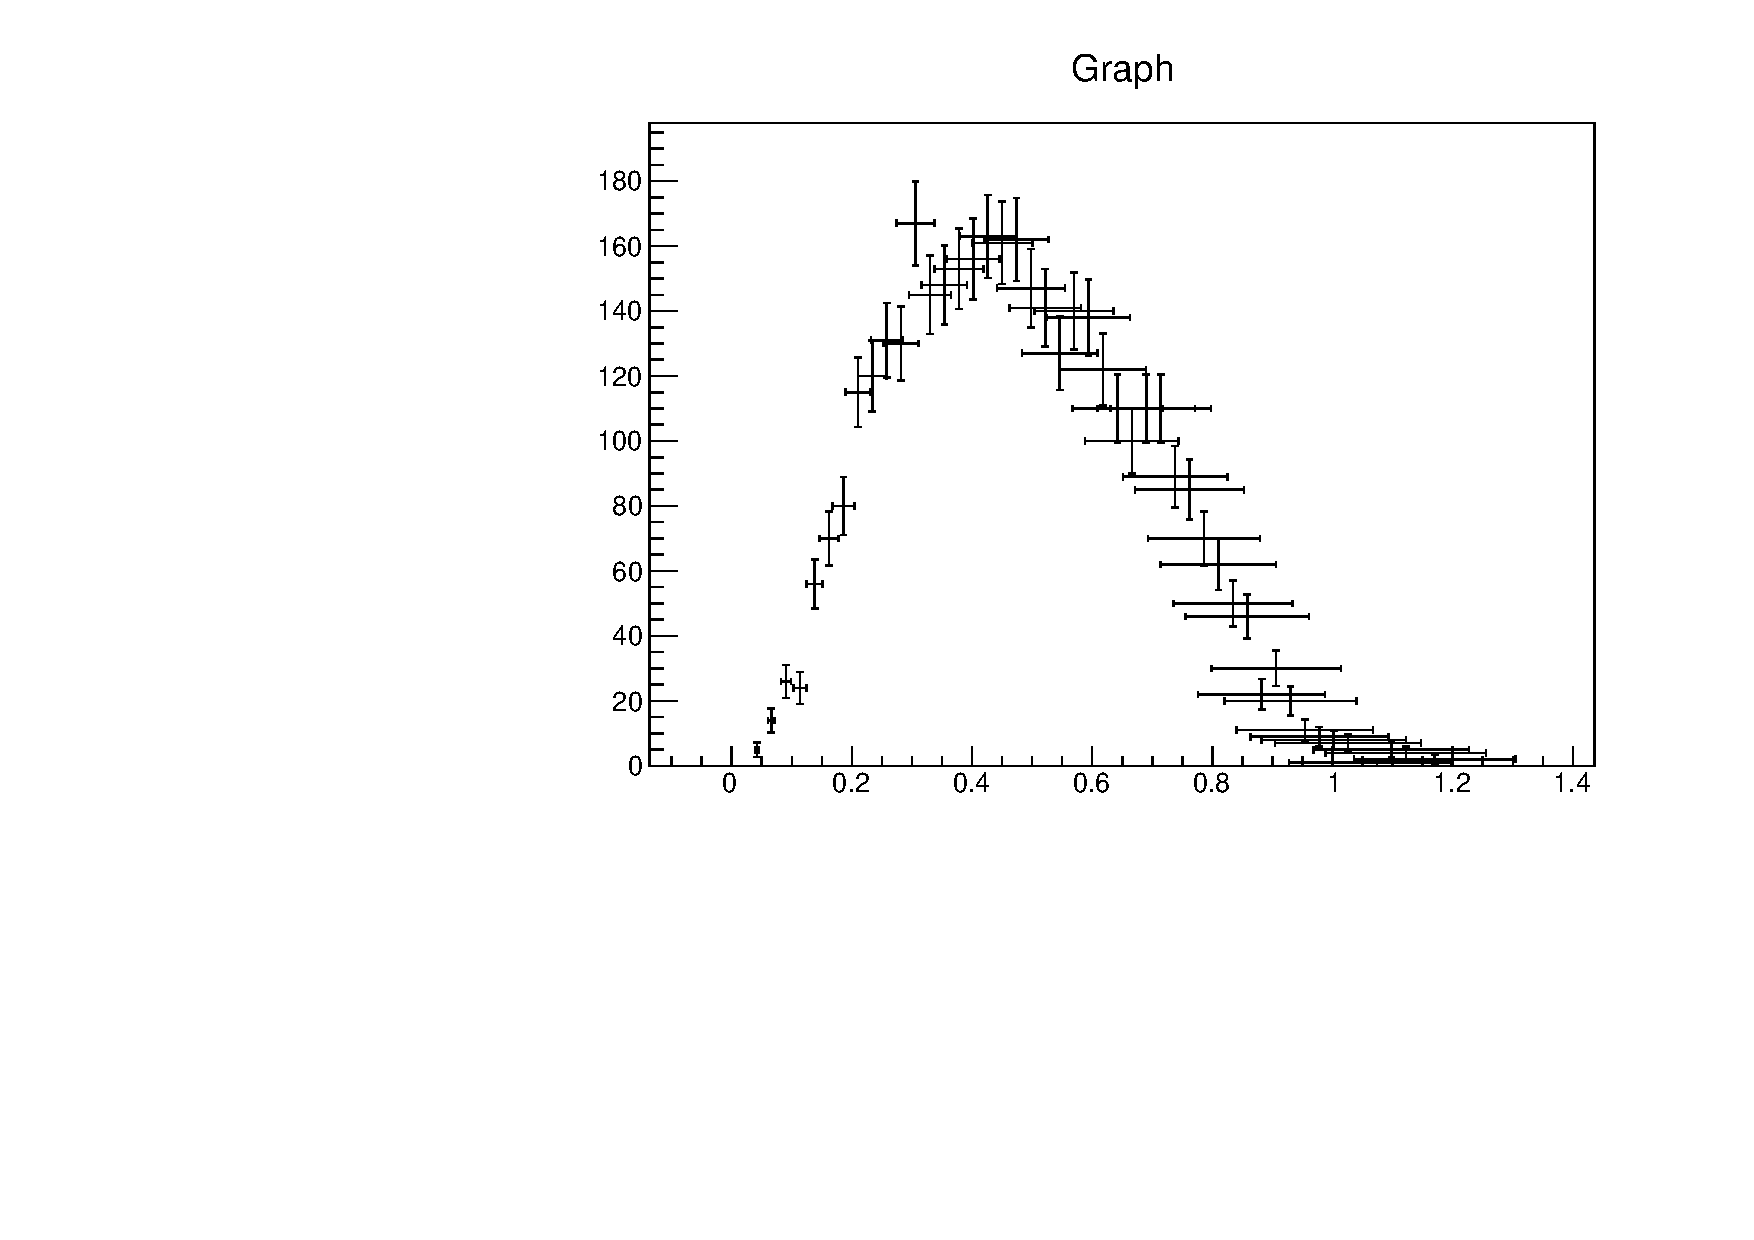
\includegraphics[height = 0.7\columnwidth , angle = -90]{figure/ikemitsu/michel_PS_gosa.pdf}
   \caption{PSで得られたエネルギー分布(誤差付き);磁場なし標的}
   \label{michel_PS_gosa}
  \end{figure}
  
  ミューオンのスピンに対して角度$\theta$の方向に崩壊する$\mathrm{e}^{+}$のエネルギー分布は,式\ref{eq:theory_michel}で与えられた.
  この式に$\rho$以外のパラメータの値として,標準模型で予想されている$\eta = 0 , \xi = 1 , \xi \delta = 3/4$を代入して計算すると,
  \begin{equation*}
   \frac{d\Gamma}{dx} \propto x^{2} [\frac{2}{3}(\rho + \frac{3}{8}\cos \theta - \frac{1}{8})(4x-3) + \frac{1}{4}(\cos \theta + 3)]
  \end{equation*}
  となる.

  図\ref{michel_PS_gosa}のグラフを$f_{\mathrm{michel}}(x) = x^{2} (A(4x -3) + B)$でfittingすることにより$\rho$を求めることができると考えた.
  しかし,高エネルギー側での横軸の誤差が大きいこともありfittingはうまくいかなかった.以下ではエネルギー解析についての課題を述べる.

  PSは無機シンチレータに比べて密度が小さいので,電磁シャワーで生じたフォトンが検出器の外側に漏れやすい.%フォトンの発生の頻度がNaIに比べて低いことも注目すべき
  これによって測定されるエネルギーが入射粒子のエネルギーよりも低くなるイベントが生じる.
  したがって測定の結果得られるエネルギー分布は入射粒子の分布と比較して高エネルギー側が少なく低エネルギー側が多い分布になる.
  %これによって高エネルギーの粒子の観測数が減ると考えられる.%観測数とはなにか?
  解析的にこの課題を解決するには,シミュレーションによって入射粒子のエネルギーと観測されるエネルギーの対応を求めてfitting関数にその寄与を組み込む必要がある.

  具体的には,シミュレーションによってあるエネルギー$E_\mathrm{incident}$をもつ粒子が入射したときの検出器中での損失エネルギー$E_\mathrm{detect}$の分布を求め,それを適当な関数で近似する.
  これを0から50 MeV の$E_\mathrm{incident}$に対して行い,得られた$E_\mathrm{detect}$の分布関数を$f(E_\mathrm{incident})$とおく.
  入射粒子のエネルギー分布$g_{\mathrm{real}}(E)$を$f(E_\mathrm{incident})$でたたみ込み積分することで,予想される分布関数$g_{\mathrm{measure}}(E)$が得られる.
  $g_{\mathrm{measure}}(E)$を用いれば測定で得られるグラフをfittingすることができると考えられる.
  %解析的にこの課題を解決するには,シミュレーションによって入射粒子のエネルギーと観測されるエネルギーの対応を求めてfitting関数にその寄与を組み込む必要がある.%それでそれに対してどうするのか?
  
  また,この実験ではPSのエネルギー較正に改善の余地が大いに残されている.
  宇宙線ミューオンを用いたキャリブレーションならば,fingerとのcoincidenceを取ることによって測定する宇宙線の飛跡を制限できる.
  こうすることで測定される宇宙線の損失エネルギーの幅は狭くなり,また,いくつかの飛跡に対してエネルギー測定を行うことで異なる損失エネルギーに対する電荷量をもとめられる.
  これらの理由から,測定する宇宙線の飛跡を制限することで較正直線の誤差を小さくすることができると考えられる.
  %宇宙線ミューオンを用いたキャリブレーションならば,NaI検出器で行っているような,fingerとのcoincidenceをとることで精度を上げることができると考えられる.
  % NaIではfingerとのcoincidenceをとるといった処理はしていない.事実誤認.

  %%%%%%%%%%%%%%%%%%%%%%%%%%%%%%%%%%%%%%%%%%%%%%%%%%%%%
  %しかし,寿命に関して表\ref{fitrange1}と表\ref{fitrange2}の1,2段目を比較すると,遅い時間側でfittingを行うと寿命が長くなっていると分かる.
  %これは,バックグラウンドなどのノイズを信号として処理しており,その影響がイベント数の少ない部分で強く出ていることによると考えることができる.
  %これを除くためには,より詳しい波形解析によってノイズとみなせる信号の性質を特定しなければならない.
  %今回の実験ではバックグラウンド計測をしなかったが,今後の課題として,ノイズ除去を目的とした解析を行う必要がある.
  %ノイズとして想定されるものには,
  %WFDを用いた実験では波形をデータとして残せるので,こうしたノイズに起因する信号を取り除くことは可能だと考えられる.
  %寿命の解析結果として,表\ref{fit_lt}と表\ref{fitrange1}・表\ref{fitrange2}の違いをfitting範囲による系統誤差に含めた.%どのように?
  %WFDを用いた実験では波形をデータとして残せるので,ノイズに起因する信号を取り除くことは可能だと考えられる.%どのようなノイズが想定されている?
  %寿命の解析結果として,表\ref{fit_lt}と表\ref{fitrange1}・表\ref{fitrange2}の違いをfitting範囲による系統誤差に含めた.%どのように?

  %$g$因子については,バックグラウンドがあっても振動の周期への影響はないと考えられる.%なぜ?
  %したがって,fitting範囲による系統誤差はないとした.

  %%%%%%%%%%%%%%%%%%%池満パート終了%%%%%%%%%%%%%%%%%%%

 %\end{document}
